\documentclass{scrreprt}
\usepackage[english]{babel}
% deutsche Umlaute
\usepackage[utf8]{inputenc}
\usepackage[T1]{fontenc}
\usepackage{lmodern}

% für das H placement Kommando bei figures:
\usepackage{float}

\usepackage{graphicx}
\usepackage{varioref}
\usepackage[
bookmarks=true,	% Lesezeichen erzeugen
bookmarksopen=false,	% Lesezeichen ausgeklappt
bookmarksnumbered=true,	% Anzeige der Kapitelzahlen am Anfang der Namen der Lesezeichen
pdfstartpage=1,	% Seite, welche automatisch geöffnet werden soll
%baseurl=http://www.server.de/dateiname.pdf, 
%  URL des PDF-Dokuments (oder Hintergrundinformationen)
pdftitle={STAV Report},
% Titel des PDF-Dokuments
pdfauthor={Johannes Schneider, Tim Henning},	% Autor(Innen) des PDF-Dokuments
%pdfsubject={},	% Inhaltsbeschreibung des
%pdfkeywords={},
% Stichwortangabe zum PDF-Dokument
breaklinks=true,	% ermöglicht einen Umbruch von URLs
colorlinks=true,	% Einfärbung von Links
linkcolor=black,	% Linkfarbe: schwarz (z.B. im Inhaltsverzeichnis)
anchorcolor=blue,	% Ankerfarbe: schwarz
citecolor=black, % Literaturlinks: schwarz
filecolor=black,	% Links zu lokalen Dateien: schwarz
menucolor=black, % Acrobat Menü Einträge: schwarz
pagecolor=blue, % Links zu anderen Seiten im Text: schwarz
urlcolor=black,	%  URL-Farbe: schwarz
%backref=true,
pagebackref=false,
pdfcenterwindow=true,
pdfnewwindow=true,
pdffitwindow=true,
pdfstartview=FitH,
pdfpagemode=UseOutlines
]{hyperref}
\usepackage{cleveref}

\usepackage{listings}
\lstdefinestyle{mystyle}{
	breakatwhitespace=false,         
	breaklines=true
}
\lstset{style=mystyle}
\lstset{
	language=C++,
	basicstyle=\ttfamily,
	keywordstyle=\color{blue}\ttfamily,
	stringstyle=\color{red}\ttfamily,
	commentstyle=\color{green}\ttfamily,
	morecomment=[l][\color{magenta}]{\#}
}
% commands to skip lines:
\lstset{numbers=left,numberblanklines=false,escapeinside={(*@}{@*)}}
\let\origthelstnumber\thelstnumber
\makeatletter
\newcommand*\Suppressnumber{%
	\lst@AddToHook{OnNewLine}{%
		\let\thelstnumber\relax%
		\advance\c@lstnumber-\@ne\relax%
	}%
}

\newcommand*\Reactivatenumber[1]{%
	\setcounter{lstnumber}{\numexpr#1-1\relax}
	\lst@AddToHook{OnNewLine}{%
		\let\thelstnumber\origthelstnumber%
		\refstepcounter{lstnumber}
	}%
}
\makeatother


\title{TAV - Report}
\subtitle{Project: Luminosus}
\author{Johannes Schneider and Tim Henning}

\begin{document}

\maketitle

\tableofcontents

\setcounter{chapter}{-1}
\chapter{Application Selection}

\section{Introduction}

Modern lighting desks used to control the stage technique in large theaters and concert halls are complex embedded system, often running a proprietary software on a Linux or Windows system in combination with two or more multitouch screens and custom hardware like faders and encoders. They are connected to all the systems in an event location like house- and stage lights, projectors, hoists and sometimes even the sound equipment. For communication between the components the industry recently started to use standardized network protocols.

Extending the functionality of such a lighting desk can be a difficult and time consuming task. To make it easier to integrate and test new features, the idea was to create a separate modular software platform that is connected via network to the lighting console. As a solution for this "Luminosus" was developed.

It is designed for lighting consoles from the market leader Electronic Theatre Controls (ETC) and uses the Open Sound Control (OSC)\footnote{see \textit{The Open Sound Control 1.0 Specification} by Matt Wright} protocol to control them. The user interface consists of modular function blocks that can be freely moved and connected. An example can be seen in \vref{fig:luminosus_example}.

\begin{figure}[h]
	\centering
	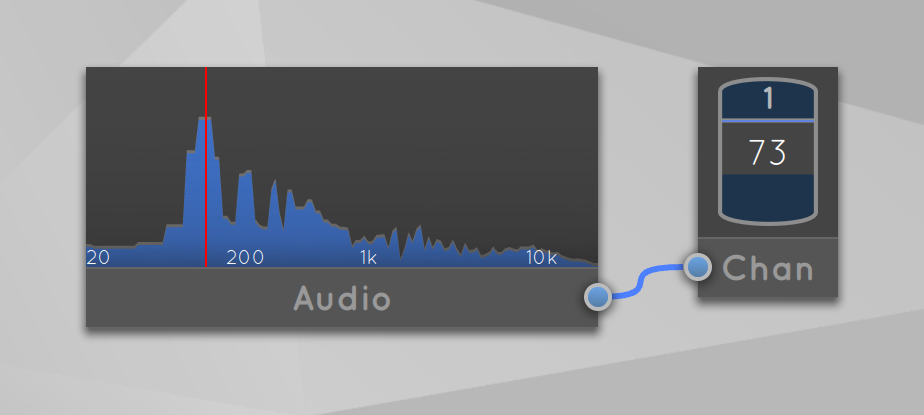
\includegraphics[width=0.75\textwidth]{img/luminosus_example}
	\caption[Luminosus Example]{Luminosus Example: Controlling the brightness of channel 73 by the current audio level}
	\label{fig:luminosus_example}
\end{figure}

The main project development was done by Tim Henning while writing his bachelor thesis. He is the only developer of the project until now. For this V\&V project Johannes Schneider joined the project as a developer and tester.

The programming language used is C++ 11 with syntax additions by Qt. The user interface part uses the declarative language QML\footnote{ sometimes referred to as 'Qt Modeling Language', see \url{http://doc.qt.io/qt-5/qtqml-index.html}} that includes function definitions in JavaScript.

The application is intended to be used by end users. It runs as a desktop application on Windows and MacOS and as an app on Android and iOS.

The existing code base consists of approximately 40k LOC (C++ source and header files + QML files). The code can be found on GitHub\footnote{\url{https://github.com/ETCLabs/LuminosusEosEdition}}.

Available artifacts are the source code, documentation, changelog\footnote{\url{https://github.com/ETCLabs/LuminosusEosEdition/blob/master/doc/Changelog.txt}}, issue tracker\footnote{\url{https://github.com/ETCLabs/LuminosusEosEdition/issues}}, manual\footnote{\url{https://github.com/ETCLabs/LuminosusEosEdition/blob/master/doc/Manual_en.pdf}} and in addition the Bachelor thesis \textit{Entwicklung einer modularen Benutzeroberfl\"ache als zus\"atzliche Bedieneinheit einer Lichtkonsole} including a requirement analysis and a discussion of the architectural decisions.

No specific development paradigm was used.

The current V\&V status is that only manual tests are performed (adding all available function blocks as a kind of \textit{smoke test} is available in the GUI) and static code analysis using Clang is provided by the IDE. Verification was not done yet.

\section{Learning from failures}

The following section is about learning from failures, which occurred over the course of developing the software.

\paragraph{Issue \href{https://github.com/ETCLabs/LuminosusEosEdition/issues/2}{\#2} Connection to Eos stopped working:}

Since the software is basically an extension for an existing hardware device, the so-called lighting console, the most important component is the network connection to the said hardware. Should this component fail to execute its duties the entire software would become useless.
That said, this exact scenario appeared for a user during his show. The connection to his lighting console was interrupted for yet unknown reasons. Furthermore, the user was not able to pick up the lost connection even after restarting his entire setup, including multiple hardware components.

Although the fault is still undetected, it can be categorized as complexity related. This is, because the interaction of different devices in various environments is very hard to predict and even harder to test upfront. Reasons for this failure range from outdated driver software for the said hardware components over defective hardware up until a fault within the networking component of Luminosus.

\paragraph{Issue \href{https://github.com/ETCLabs/LuminosusEosEdition/issues/3}{\#3} Faders not updated:}

The Eos lighting console offers a set of faders to control the light intensity on different devices. But since this set is very limited in the amount of supported devices, Eos additionally includes virtual pages of faders. Thus, the effective amount of hardware one can manage using the Eos lighting console increases immensely.

Luminosus also offers the feature of switching pages of faders. 

\begin{figure}[H]
	\centering
	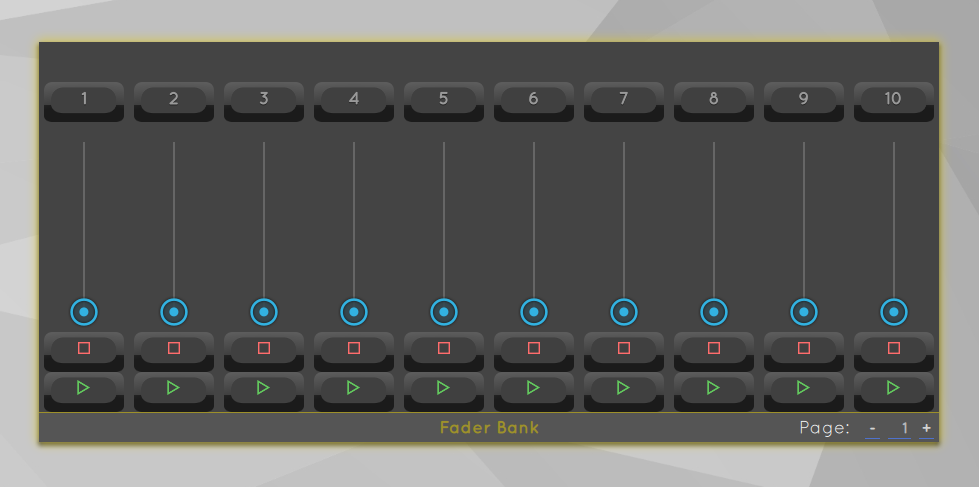
\includegraphics[width=0.75\textwidth]{img/luminosus_faders}
	\caption[Luminosus Fader Bank]{Luminosus Fader Bank: Visualization of the Eos faders including virtual pages}
	\label{fig:luminosus_faders}
\end{figure}

However, when switching between these pages, the corresponding faders were not updated properly. To be exact, they were not updated at all.

This failure was caused by a single missing line, which sets all faders to their initial position before requesting their current state. Thus, the fault was preventable, since a simple unit test could have covered this functionality.


\paragraph{Issue \href{https://github.com/ETCLabs/LuminosusEosEdition/issues/4}{\#4} Fullscreen on iOS not working:}

Luminosus is designed to be cross-platform compatible. Thus, when working on a desktop computer most users would like Luminosus to be presented in fullscreen mode. This wish was realized by implementing a button, which offers just this functionality.
However, when running Luminosus on iOS, the fullscreen button caused the UI scaling to increase. This rendered the software practically unusable.

The exact cause for this failure is not discovered yet. Still you could say this failure was preventable by having a unit test which compares the scale property before and after the operation. However, the fault could also be treated as intelligent related, since the button should have not been enabled for mobile devices in the first place. So even if the function would have been working as expected, the resulting behavior would be irritating as the only difference of the fullscreen mode on a mobile OS is the removal of the status bar, which does not help the user at all.

\paragraph{Conclusion}
In general the introduction of unit tests would be a valuable addition to the existing code base. Furthermore, integration tests for typical user scenarios would help to prevent many kinds of faults. Last but not least we learned that to maintain so many different platforms the user feedback is an important part in the process of V\&V.


\section{Five Basic V\&V Questions}

\paragraph{When do V\&V start?  When are they complete?}

Validation started right in the beginning. The project was validated on a daily basis  due to a lot of contact to the supervisor. The specification was adjusted very frequently to ensure that the features that were developed were suitable for the projects goal.

Analysis began early, too, in the form of static code analysis provided by the IDE (Qt Creator) and Clang. The development of tests did not start until the beginning of this V\&V lecture.

The process of V\&V does not end until the end of the lifetime of the product. In this case as long as the software is maintained.

\paragraph{What particular techniques should be applied during development?}

Static code analysis is very good applicable for C++ due to strict type declarations. 

Continuous Integration should be applied to the project since it will be used on various platforms. Furthermore, automated unit testing will be applied during the semester.

Additionally, profiling the memory consumption can help finding memory leaks and performance benchmarks make sure that the specification is met in terms of latency and responsibility.

In the end a formal verification of standardized components such as the network protocol implementations should be applied.

\paragraph{How can we asses the readiness of the product?}

The readiness is assessed by using the defined features of the specification and their current implementation status. Before a release is considered ready it should be at least tested manually in a typical use case scenario.

Furthermore, open issues are a hint that the product is not yet ready.

In the end the validation of a product is easier when the developer is also a user, as in our case. The greater the distance of the developer to the users of the product, the harder it is to match the use cases with the implementation. 

\paragraph{How can we control the quality of successive releases?}

To ensure that successive releases do not introduce new faults a pre-release policy can be established to let a small group of beta users test the system before it is released to the public.

The successful run of automated tests, especially regression tests, in a Continuous Integration environment can be a good indicator too.

\paragraph{How can the development process itself be improved?}

Increasing emphasis on applying various V\&V techniques during further development will help to improve overall code quality. 

Furthermore the development process can be improved by introducing a second developer to the project. Thus, pair programming and code reviews can be established to help finding flaws. In addition maintaining the documentation will lead to a better process.


\chapter{Analysis}

\section{Human-based Static Analysis}

The following section of about the peer review we performed. We figured out advantages and weaknesses of this technique.

\subsection{Peer Review}
\label{subsec:peer_review}

We organized our peer review sessions by picking suitable code snippets for each other. These snippets were supposed to be readable, even for someone who is not as deeply involved in the project or even the programming language at all. We then presented the selected code to the other group, while also introducing the general project. Afterwards, we further increased our understanding by asking questions about unclear syntax or general questions about details within the code. Finally, we were able to discuss issues and tried to find suitable solutions.

The code snippet we prepared is shown below.

\bigskip
\begin{lstlisting}[language=C++,
					numbers=left,
					firstnumber=171,
					directivestyle={\color{black}}
					emph={int,char,double,float,unsigned},
					emphstyle={\color{blue}},
					title=src/eos\_specific/EosCue.cpp]
void EosCue::createCueBlock() {
  EosCueBlock* block = qobject_cast<EosCueBlock*>(m_controller->blockManager()->addNewBlock("Eos Cue"));
  if (!block) {
    qWarning() << "Could not create Cue Block.";
  }
  block->setCueNumber(m_cueNumber);
  block->focus();
}
\end{lstlisting}
\bigskip

As requested, the code contained a fault. This fault was to be detected by our partners for the sake of this peer review.
The fault was a missing \texttt{return}-statement after line 174. This caused the function to continue its execution even when the \texttt{block} is a \texttt{nullptr}. Consequentially, line 176 would try to dereference this invalid pointer thus causing most likely an uncaught exception leading to a termination of the software.

After only a short while, our partners were able to locate and also fix the mentioned defect.

In return, they had a code snippet prepared for us which included a defect as well. 

% TODO: include code

When we finished understanding the context and general idea of the presented code, we were able to find the defect. Furthermore, we also suggested a change in the documentation, since it was misleading.

All together, our peer review session was mainly used for communication purposes and understanding the projects of each other. Additionally, the peer review helped us to exchange thoughts about various faults not only within our group but also with members of our partners group.

Main advantage of this kind of peer review is the fact, that every code snippet can be discussed directly with its author. This enables a very deep discussion about certain implementation decisions and also improves the overall code understanding by far. After just a short while, we were even able to detect a misleading documentation for a certain implementation, although we never saw the code before. 

In general, peer reviews can help to improve the product by selecting difficult code and talking about it in a very objective way. Thus, we do not need to play the blaming game and can just focus on finding and avoiding faults for future implementations. Additionally, it is very important to do this kind of analysis on a regular basis, so that the reviewed code is still manageable in size and difficulty. 

\subsection{Tools}

When performing peer reviews in a more professional way than we did, companies often use tools to support their process. The following section will evaluate some of the tools we already used.

\subsubsection{GitHub}

A tool we are very comfortable using is GitHub\footnote{\url{https://www.github.com}}. GitHub does not only allow you to host git repositories, so all your code is in just one place, but also offers a great variety of reviewing tools, like commenting coding line by line (see \vref{fig:github_review_comment}). The concept of pull requests and its support is also a very strong feature in GitHub. It offers developers a very formal way of merging branches into each other. It supports a human based review process by naming one or more reviewers for the pull requests. These reviewers may then comment, ask questions or suggest improvements for the code at hand. Although this process is mostly covered by the features offered by GitHub, we would like to have a way of (autonomously) selecting code of interest as we did in our peer review. Right now, every reviewer has to read all the code submitted for merging, making it very time consuming.

\begin{figure}[h]
	\centering
	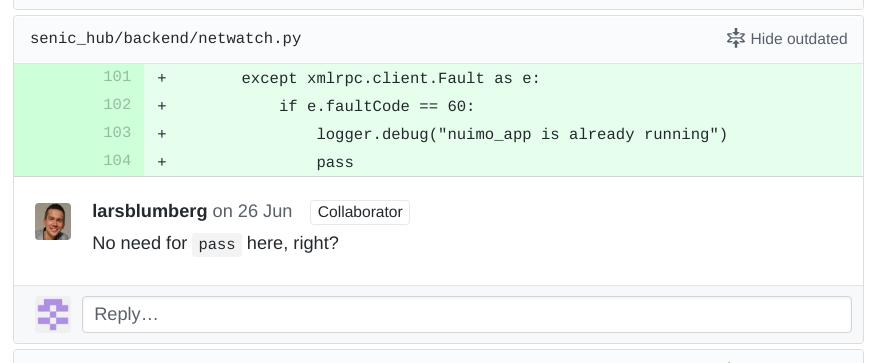
\includegraphics[width=0.9\textwidth]{img/github_review_comment}
	\caption[GitHub Review Comment]{A comment in the GitHub review tool}
	\label{fig:github_review_comment}
\end{figure}

While it is comfortable for the team members that these functions are integrated into the GitHub website and work in every browser, this also means that no code exploration features known from various IDEs are available. As a beginning it would be nice, for example, to be able to jump to a function declaration right from the review page of GitHub. This would help understanding the code a lot.

\subsubsection{SonarQube}

Besides GitHub, SonarQube\footnote{\url{https://www.sonarqube.org}} is another excellent web based tool for reviewing code. In contrast to GitHub, SonarQube is not used as a repository host. What makes SonarQube still great is its build-in fault detection and static analysis. Thus, a reviewer can find any flaws very fast and also see, who authored the corresponding code. We will cover more of the automated static analysis feature of SonarQube in section \ref{sec:humand-based-vs-automated-sa}.

What we missed when we used SonarQube was the possibility to see the entire commited code at once. SonarQube only offers to jump to fault it detected, but has no possibility to see the entire commit.

\section{Automated Static Analysis}

After we discovered and tested the human-based analysis of code, we also wanted to try automated analysis. Therefore, we chose tools, which are commonly used when analyzing C++ code. Our findings are documented in the following section.

\subsection{Clang Static Analyzer}

The first tool we tested was the Clang Static Analyzer\footnote{\url{https://clang-analyzer.llvm.org}}. We decided to test this tool not only because it has a great plugin for the IDE of our choice (Qt Creator\footnote{\url{https://www.qt.io/}}), but also because it is around for quite a while and therefore commonly known in the C++ community.

On the one hand, Clang helped to improve the code by finding a possible nullpointer dereference caused by a missing return statement (see \vref{subsec:peer_review}). 
On the other hand it reported hundreds of false alarms in its default configuration, i.e. increase of precision of floating point numbers thereby making it harder to detect the real faults (see \vref{fig:clang_fp_implicit_precision_increase}).

\paragraph{Inaccuracy}

The developers of Clang Static Analyzer clearly stated that the tool was made to reported as less false positives as possible. However, they are more concerned about not finding a fault, so they would tolerate a moderate amount of false alarms. This leaves us with the conclusion that the Clang Static Analyzer is mainly incorporating pessimistic inaccuracy, which results in false alarms. However, the tool can be configured to also include optimistic inaccuracy, if needed. This can be realized by adding filters so that some checks will become less strict. This behavior will result in some faults not being detected any longer.

\begin{figure}[H]
	\centering
	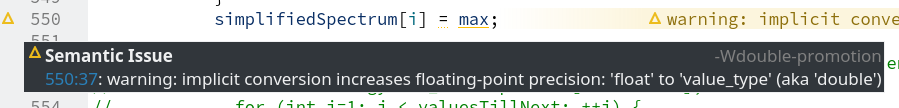
\includegraphics[width=0.9\textwidth]{img/clang_fp_implicit_precision_increase}
	\caption[Clang warns of increase in precision]{Clang warns of increase in precision of floating point number}
	\label{fig:clang_fp_implicit_precision_increase}
\end{figure}

Figure \ref{fig:clang_fp_implicit_precision_increase} is an example, of a very strict default configuration which leads to a false positive in our concrete project.

\subsection{Clang-Tidy} 

Next to the Clang Static Analyzer there is also the command line tool clang-tidy\footnote{\url{http://clang.llvm.org/extra/clang-tidy/}}. The tools are quite similar, the static analyzer focuses more on checks that require some sort of control flow analysis while clang-tidy includes linter-style checks and checks that are related to a certain coding style\footnote{see discussion here: \url{http://lists.llvm.org/pipermail/cfe-dev/2015-September/044966.html}}. Other than the static analyzer, clang-tidy is able to automatically fix most of the issues it found by modifying the source files directly, which is a very powerful feature to modernize legacy code bases.

In our case, clang-tidy was able to point out some hard to find readability issues such as a misleading use of static\_cast where dynamic\_cast would be more appropriate because it was a downcast from a base to a derived class. It also suggested good uses for the auto keyword, missing \texttt{override} keywords and showed function definitions where the variable names did not match those of the declaration. It even highlighted a case where a function call contained an inline comment with the name of the parameter (like '\texttt{foo(/*parameterName=*/ true)}') that did not match the real parameter name. After a quick configuration we were able to suppress most of the warnings related to a different coding style resulting in mostly true positives were shown.

\subsection{CppCheck} 

Although CppCheck\footnote{\url{http://cppcheck.sourceforge.net}} found faults which Clang missed, such as uninitialized member variables, we more disappointed for the most part. This is, because CppCheck claims to be designed to show as less false positives as possible, but still displayed a huge bunch of them for our project (see \vref{fig:cppcheck_fp_missing_ctor}).

\begin{figure}[h]
	\centering
	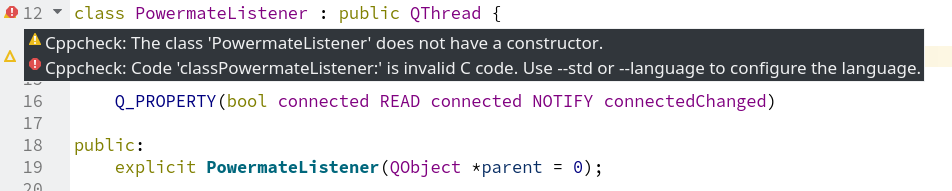
\includegraphics[width=0.9\textwidth]{img/cppcheck_fp_missing_ctor}
	\caption[Bugs in CppCheck]{Bugs in CppCheck result in false positives}
	\label{fig:cppcheck_fp_missing_ctor}
\end{figure}

This unwanted behavior is most likely caused by a bug in CppCheck itself, making it even more unsatisfying to use this tool in the first place.

\paragraph{Inaccuracy}

According to their website, the goal of CppCheck is to have zero false positives, resulting in a low pessimistic inaccuracy. They even recommend to use an additional tool that has a greater pessimistic inaccuracy, if required for the project. Unfortunately, in practice there are still some false positives, mainly related to bugs in CppCheck, as already mentioned before. The developers state that there are many faults that are not detected by CppCheck which leads to a high optimistic inaccuracy.

\subsection{Polyspace} 

Other than the previously shown tools, Polyspace\footnote{\url{https://www.mathworks.com/products/polyspace.html}} is a commercial product, which is made for industry standards of security critical environments. It claims to be capable of handling huge amounts of code and is also able to apply very in-depth analysis techniques, such as proofing the absence of some types of faults, like buffer overflows, division by zero and wrong array accesses\footnote{see \url{https://www.mathworks.com/products/polyspace-code-prover.html}}.

In the preparation of this report we tried to apply this tool to our project, but experienced some problems in using it (see \vref{fig:polyspace_analysis}). We were only able to validate one single source file, the only file with no dependencies other than the C++ standard library. To resolve the Qt includes, it would be necessary to monitor the build process of the project by Polyspace, which was not possible due to limited access to the system where Polyspace was installed on.

\begin{figure}[h]
	\centering
	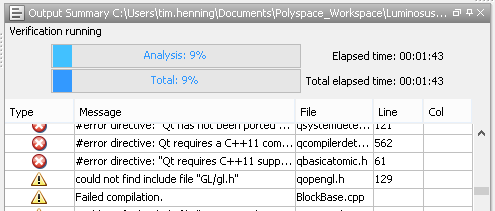
\includegraphics[width=0.7\textwidth]{img/polyspace_analysis}
	\caption[Polyspace Analysis]{Polyspace showing errors while analyzing C++ code with Qt dependencies}
	\label{fig:polyspace_analysis}
\end{figure}

\paragraph{Inaccuracy}

Polyspace is the only tool that we evaluated which claims to have zero optimistic inaccuracy for a specific set of faults. It realizes this by abstract interpretation of the code and automated formal validation methods.

\subsection{CppLint} 

A tool that is specialized in style guide checks is Googles cpplint.py\footnote{\url{https://github.com/google/styleguide/tree/gh-pages/cpplint}}. Even while this projects style guide differs from Googles, the tool can give some interesting hints. As an example, it was able to find missing includes that the other tools did not report. This is a valuable addition and shows again, that in the case of automated static analysis it is better to use a bunch of tools instead relying on a single one.

\section{Interaction between Human-Based and Automated SA}
\label{sec:humand-based-vs-automated-sa}

\begin{figure}[h]
	\centering
	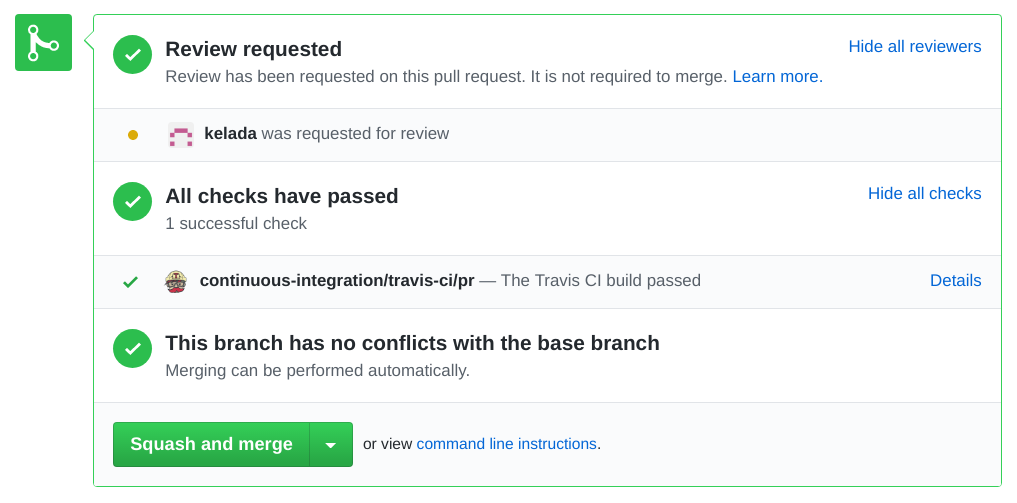
\includegraphics[width=0.9\textwidth]{img/github_pr_review}
	\caption[GitHub PR review]{Combination of ASA and human-based reviews in GitHub}
	\label{fig:github_pr_review}
\end{figure}

By using ASA a peer review can be prepared in order to point out potentially broken code parts. It can then be discussed if a detected fault is considered a false positive or not, and how to fix it. Additionally, some faults might be caused by a bad habit within the project team. These faults are very interesting to discover and can indicate certain lacks of the developing team, enabling more overall awareness once discussed thoroughly. They might even cause a change in the general consideration of good code in the team.  

When using tools like SonarQube, the faults get matched with their author. This enables each developer to learn from their mistakes in a more direct way. Additionally, it also displays which kind of faults are often produced in a project. These faults can then be targeted by further education and more awareness.

When thinking the other way around, the results of a human-based peer review can be used to improve the configuration of the automated static analysis tools. This can reduce the number of false positives which are caused by the coding guidelines of the individual project and thus are intended.
Depending on the use case, the relevance of faults is differently prioritized. In our specific case the implicit increase of precision of floating point numbers is not a problem at all. In contrast, in more space critical applications this could lead to unpredictable behavior.

In addition to the combination of ASA and human-based reviews, testing can also be integrated in this process. GitHub is a good example for this, as it shows the result of different software verification and validation methods at one glance, as seen in \vref{fig:github_pr_review}.

\chapter{Testing}

\section{Kick-off Tasks}

\subsection{Example Test Set}

As an example bug we chose issue \#17\footnote{\url{https://github.com/ETCLabs/LuminosusEosEdition/issues/17}}. It describes a problem where the application sometimes crashes when receiving cue objects. The following lines of code caused this:

\bigskip
\begin{lstlisting}[language=C++,
							numbers=left,
							firstnumber=78,
							directivestyle={\color{black}}
							emph={int,char,double,float,unsigned},
							emphstyle={\color{blue}},
							title=src/OSCNetworkManager.cpp]
void onIncomingEosMessage(const EosOSCMessage& msg) {(*@\Suppressnumber@*)
    [...](*@\Reactivatenumber{92}@*)
    } else if (msg.path().size() <= 5) {
        // this message contains detailed information about a cue
        EosCueNumber cueNumber = EosCueNumber(msg.pathPart(2), msg.pathPart(3), msg.pathPart(4));(*@\Suppressnumber@*)
        [...](*@\Reactivatenumber{1}@*)
\end{lstlisting}
\bigskip

\subsubsection{Test-Case \#1}
\label{test-case-1}

The first test case should be designed to not only reach the fault but also produce the failure.

\begin{itemize}
	\item[] \underline{Test Value}
	
	An \texttt{EosOSCMessage} object, where \texttt{path().size()} equals 4.
	
	\item[] \underline{Expected Output}
	
	The application should dispose the message, since its too short.
	
	\item[] \underline{Fault}
	
	The fault is persisted in line 94, when \texttt{msg.pathPart(4)} is accessed. In our test case, this statement would access unallocated memory, leading to the \texttt{SegmentationFault}.
	
	\item[] \underline{First Error State}
	
	The first error state is reached, as soon as the \texttt{if-statement} in line 92 is evaluated to \texttt{true}. Consequentially, this leads to the execution of the following block, thus producing the fault.
	
	\item[] \underline{Failure}
	
	The failure shows exactly as the expected output. The program crashes, leaving an unresolved \texttt{SegmentationFault}.
\end{itemize}

\subsubsection{Test-Case \#2}
\label{test-case-2}

The second test case should not reach the fault at all.

\begin{itemize}
	\item[] \underline{Test Value}
	
	An \texttt{EosOSCMessage} object, where \texttt{path().size()} equals 6.
	
	\item[] \underline{Expected Output}
	
	The program continues processing the message, as specified by the protocol.
	
	\item[] \underline{Fault}
	
	The fault is still the same as in \vref{test-case-1}. However, since the \texttt{if-statement} in line 92 evaluates to \texttt{false} the fault is not reached.
	
	\item[] \underline{First Error State}
	
	-
	
	\item[] \underline{Failure}
	
	-
\end{itemize}

\subsubsection{Test-Case \#3}
\label{test-case-3}

The third test case is designed reach the fault while not producing an error.

\begin{itemize}
	\item[] \underline{Test Value}
	
	An \texttt{EosOSCMessage} object, where \texttt{path().size()} equals 5.
	
	\item[] \underline{Expected Output}
	
	The program reaches the fault, but does not produce an error. Thus, the message is processed according to the specification.
	
	\item[] \underline{Fault}
	
	The fault remains as described in \vref{test-case-1}. 
	
	\item[] \underline{First Error State}
	
	This test case does not produce a first error state. This is, because line 94 accesses only valid elements of \texttt{msg.path()}.
	
	\item[] \underline{Failure}
	
	-
\end{itemize}

\subsection{Type of Existing Test Set}

There is no existing test set. In the past, only manual testing and partly automated "monkey testing" was performed. A beta phase before releases was used to integrate the feedback from user testing.

\subsection{Different Scopes of Test Case Execution}

The following section will demonstrate, how small, medium and big tests can be applied to our project.

In order to do so, we choose to test following code snippet.

\begin{lstlisting}[title=src/OSCNetworkManager.cpp]
/*
Extracts one valid OSC packet from the given buffer. 
The packet will then be removed from the buffer and is returned as QByteArray.
*/
QByteArray OSCNetworkManager::popPacketLengthFramedPacketFromStreamData(QByteArray& tcpData) const {
	[...]
}
\end{lstlisting}
\bigskip

As described in the documentation, this method will extract and remove a valid OSC packet from the given buffer (\texttt{tcpData}) and returns this packet as \texttt{QByteArray}.

This piece of code is especially interesting for our project, as it can be tested on multiple scope sizes as follows:

\subsubsection{Small Testing}

For small testing, the method is tested isolated (e.g. without any context). We can apply different testing strategies for this method:

\begin{itemize}
	\item[] \underline{Specification Testing} % TODO: better: Validation Testing?
	
	\begin{itemize}
		\item[] \underline{Test Value}
		
		A buffer (\texttt{tcpData}), which contains exactly one valid OSC packet.
		
		\item[] \underline{Expected Output}
		
		A valid \texttt{QByteArray}, which contains all data of the given buffer. Additionally, the given buffer must be empty.
	\end{itemize}

	\item[] \underline{Defect Testing}
	
	\begin{itemize}
		\item[] \underline{Test Value}
		
		A buffer (\texttt{tcpData}), which does not contain a valid OSC packet.
		
		\item[] \underline{Expected Output}
		
		An empty \texttt{QByteArray}. Additionally, the buffer is not modified.
	\end{itemize}
\end{itemize}

These are only two examples, which do not complete any coverage criteria. Thus, the set of test cases should be expanded in the future. However, as for demonstrating how this method can be used to create small tests, these examples should be perfectly fine.

\subsubsection{Medium Testing}

For medium testing we added a little more context to the shown method. This will lead to a longer stack trace, as more methods are involved. One way of expanding the system under test is shown below:

% TODO: Verständlichkeit anheben! Warum stellen wir das Diagramm dar, was wird genau dargestellt?
\begin{figure}[h]
	\centering
	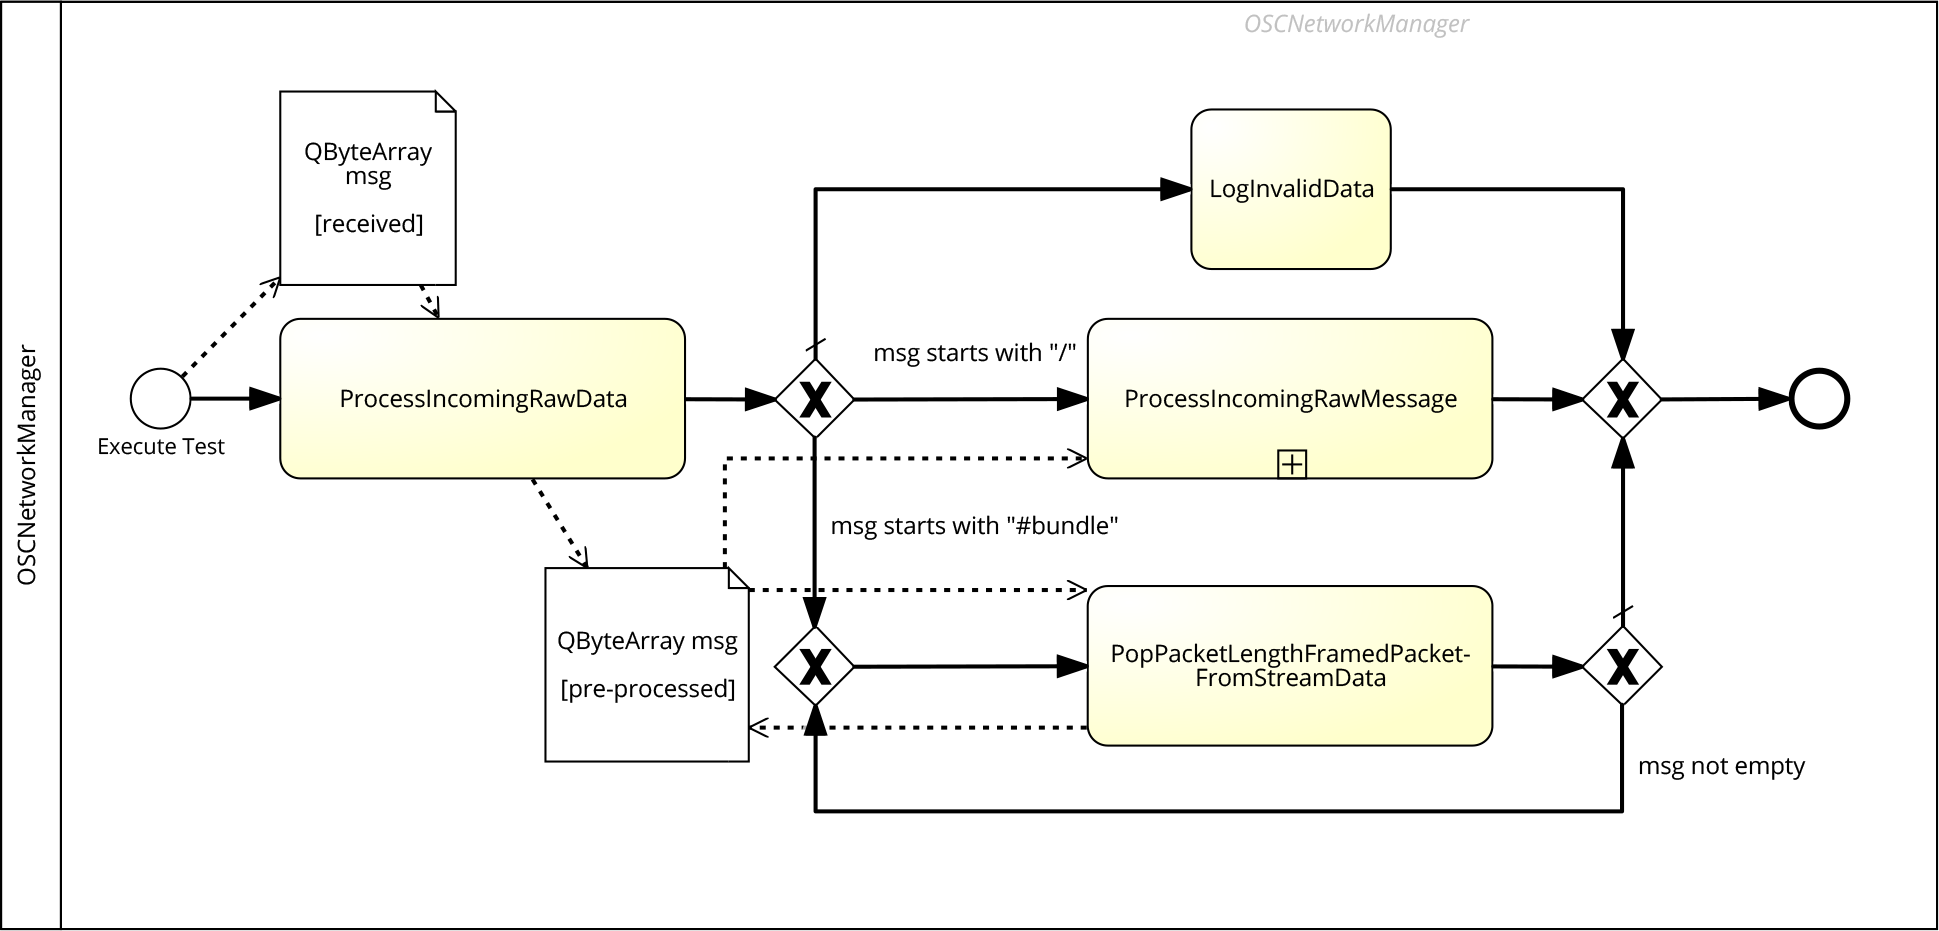
\includegraphics[width=1.1\textwidth]{img/2_1_3_medium_test}
	\caption[Medium Testing Context]{Testing context on a medium scale}
	\label{fig:medium_test}
\end{figure}


When testing the displayed context, we need start testing the method \texttt{void OSCNetworkManager::processIncomingRawData(QByteArray msgData)}. Thus, we span a call graph as shown in \vref{fig:medium_test}. The edges can be reached by manipulating the \texttt{msg} input parameter.

One method to develop test cases for our scenario is to define subsets for our input domain. To be concrete, we divided the input domain as follows:

\begin{itemize}
	\item \texttt{msg} is empty
	\item \texttt{msg} is not empty
	
	\begin{itemize}
		\item \texttt{msg} starts with \texttt{"/"}
		\item \texttt{msg} start with \texttt{"\#bundle"}
	\end{itemize}
\end{itemize}

When using this input domain subsets, we can define a test set, which covers every edge of the call graph. For evaluation of the test results we need to use a human oracle, as the concrete expected behavior depends heavily on the input data and can not be verified by specification.

\subsubsection{Big Testing}

As for big testing, we decided to replace the synthetic \texttt{msg} object from \vref{fig:medium_test} with the real network adapter. This allows us, to also include other components, which are depending on the networking module.

In order to execute tests on this scope, a real TCP connection (e.g. a TCP client, which uses the running application as its server) is needed. Using this setup, we would like to perform defect testing mainly. This is, because including hardware (such as the networking card) on a real network configuration might lead to unexpected behavior, which is otherwise hard to test. Concrete, we would like to test various things on our entire networking subsystem, like packet fragmentation, packet loss and the behavior when connections are closed unexpectedly. % TODO: add explanation why this is difficult

\section{Test Case Development}

There are multiple different approaches to generated test values for a specific test case to reach a certain kind of coverage. We will discuss some of them the following sections, using the \texttt{ColorMatrix::rescaleTo()} method as an example.

\subsection{Input Domain Modeling}

TODO

%TODO

\subsection{Logic Expressions}

Logical expression coverage is another criterion to create test cases for a certain part of code. It aims at finding bugs and unexpected behavior by not only executing each branch of code but also evaluating all clauses in conditions separately. This is not guaranteed by other coverage criteria because short-circuiting conditions may not evaluate all their clauses, even if there are test cases for the true and false cases.

We will design test cases for logical expression coverage based on the condition in the code shown in \vref{lst:logical_expression_code}.

The individual clauses are:\\
$
a = indexChangedDuringTouch\\
b = isTap\\
c = dropDownItem\\
$

The predicate is $a \lor (\lnot b \land c)$.

\bigskip
\begin{lstlisting}[language=C++,
					numbers=left,
					firstnumber=123,
					directivestyle={\color{black}}
					emph={int,char,double,float,unsigned},
					emphstyle={\color{blue}},
					caption=qml/CustomControls/ComboBox2.qml,
					label=lst:logical_expression_code]
// if the index changed
// or if it was not a tap and there is a DropDown item:
if (indexChangedDuringTouch || (!isTap && dropDownItem)) {
	// destroy the DropDown:
	dropDownItem.destroy();
}
\end{lstlisting}
\bigskip

\paragraph{Predicate Coverage (PC)}

Predicate coverage is reached by finding test cases where the logical expression, the \textit{predicate}, is at least once true and false.

To find suitable test cases we can use the truth table shown in \vref{tab:cacc}. One test case where the predicate is true (1, 2, 3, 4 or 7) and one where it is false (5, 6 or 8) is enough to satisfy PC, i.e. the test cases 1 and 8.

\paragraph{Clause Coverage (CC)}

For clause coverage it is required that each clause of the expression evaluated in at least one test case to true and false. Many test sets would fulfill this requirement, like (2, 7) or (3, 6). The test set (1, 8) has the additional benefit that it also satisfies predicate coverage.

\paragraph{Correlated Active Clause Coverage (CACC)}

Correlated Active Clause Coverage, where each clause is tested independently, can be reached by choosing one pair of (1, 5), (2, 6) or (3, 8) for the major clause $a$, the test cases (5, 7) for the major clause $b$ and (7, 8) for the major clause $c$.

A minimal test set that satisfies PC, CC and CACC would then be (1, 5, 7, 8).

\paragraph{Combinatorial Coverage (CoC)}

The most comprehensive coverage criterion for logical expression based testing is to test all combinations of truth values of each clause. This needs $2^N$ tests, with $N$ being the number of clauses. All 8 combinations are shown in \vref{tab:cacc}. 

\begin{table}[h]
	\centering
	\caption{\label{tab:cacc}Correlated Active Clause Coverage (CACC)}
	\begin{tabular}{r|ccc|c|l|c|c}
		   & $a$ & $b$ & $c$ & $a \lor (\lnot b \land c)$ & $p_a$ & $p_b$ & $p_c$ \\ \hline
		1 & T & T & T & T & *\quad\quad  &   &  \\
		2 & T & T & F & T & \quad*\quad  &   &  \\
		3 & T & F & T & T & \quad\quad*  &   &  \\
		4 & T & F & F & T &        &   &  \\
		5 & F & T & T & F & *\quad\quad  & * &  \\
		6 & F & T & F & F & \quad*\quad &   &  \\
		7 & F & F & T & T &        & * & *  \\
		8 & F & F & F & F & \quad\quad* &   & *  \\
	\end{tabular}
\end{table}

\subsection{Control Flow Graph}

\begin{figure}[h]
	\centering
	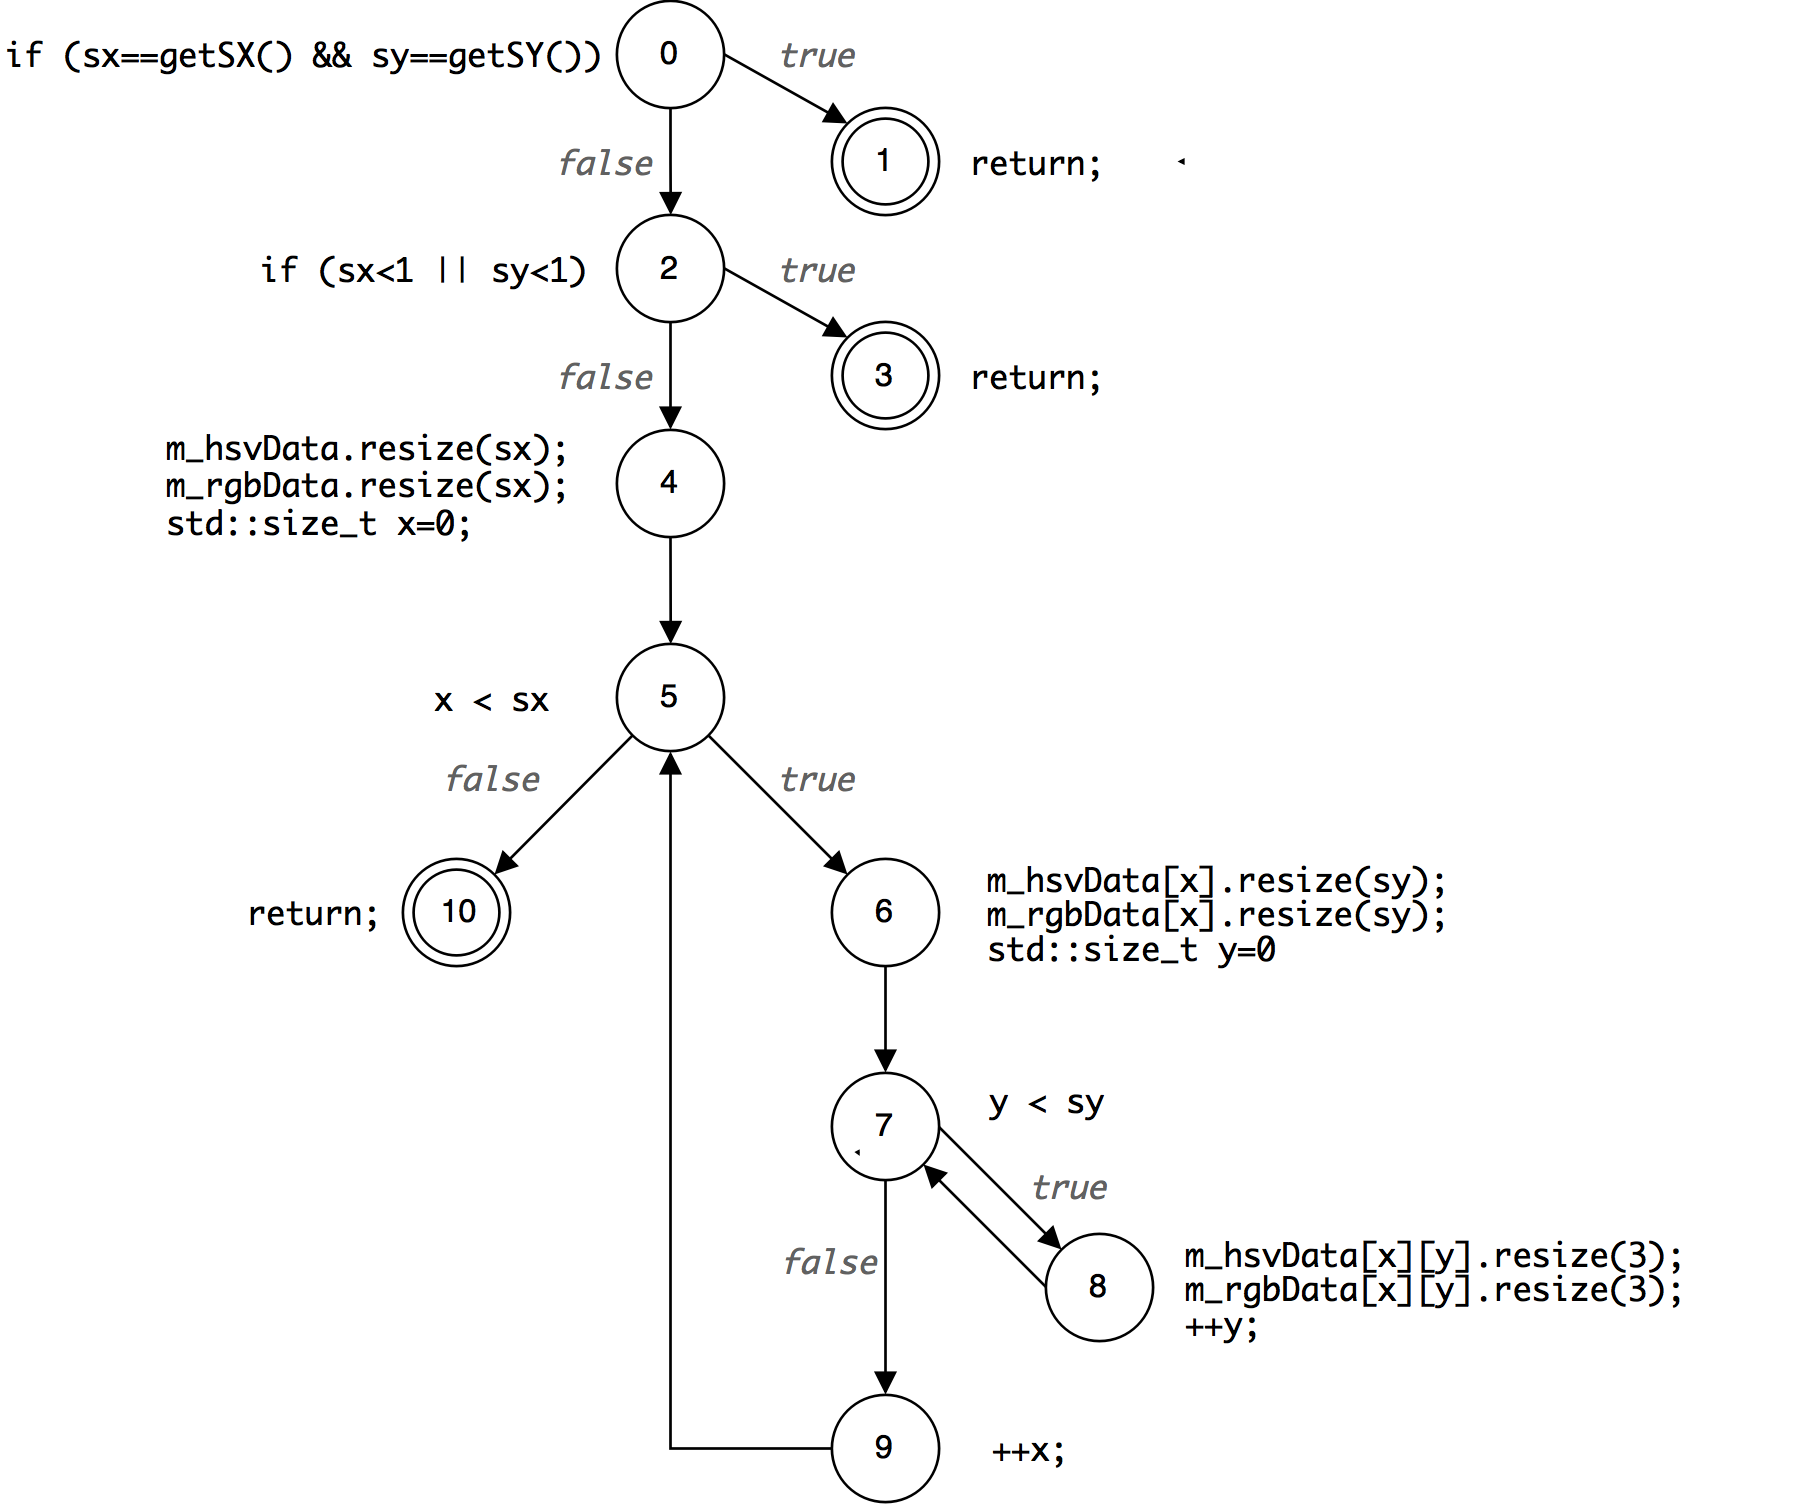
\includegraphics[width=1.0\textwidth]{img/cfg_rescale_to}
	\caption[Control Flow Graph rescaleTo()]{Control Flow Graph of the rescaleTo() Method}
	\label{fig:cfg_rescale_to}
\end{figure}

\paragraph{Node Coverage} The simplest way to cover a control flow graph as seen in \vref{fig:cfg_rescale_to} is to create test cases that visit all nodes at least once. For the rescaleTo() method three paths have to be covered for this: (0, 1), (0, 2, 3), (0, 2, 4, 5, 6, 7, 8, 7, 9, 10).

The four input parameters that rescaleTo() depends on, are the current width and height of the matrix and the parameter of the function sx and sy. To execute the three mentioned paths the following input values can be used: [1, 1, 1, 1], [1, 1, 0, 0], [2, 2, 1, 1].

\paragraph{Edge Coverage} The same test values can be used to reach edge coverage, i.e. visit all edges of the graph at least once.

\paragraph{Edge Pair Coverage} To cover all pairs of edges, two additional paths would have to be covered. The path (0, 2, 4, 5, 10) is infeasible because the second if-statement makes sure that the rest of the method is only executed when the size changes, which means the for-loops are executed every time node 4 is reached.
The path (0, 2, 4, 5, 6, 7, 8, 7, 9, 10) is expanded to (0, 2, 4, 5, 6, 7, 8, 7, 8, 7, 9, 5, 6, 7, 8, 7, 8, 7, 9, 5, 10) to also cover the edge pair (9, 5, 6). This path is executed with the input values [2, 2, 1, 1].

\paragraph{Prime Path Coverage} The following prime paths were calculated with the online tool by Ammann and Offutt\footnote{\url{https://cs.gmu.edu:8443/offutt/coverage/GraphCoverage}}:

\begin{itemize}
	\item[a)] 0, 1
	\item[b)] 0, 2, 3
	\item[c)] 0, 2, 4, 5, 10
	\item[d)] 0, 2, 4, 5, 6, 7, 8, 7, 9, 5, 10
	\item[e)] 0, 2, 4, 5, 6, 7, 8, 7, 8, 7, 9, 5, 10
	\item[f)] 0, 2, 4, 5, 6, 7, 9, 5, 6, 7, 8, 7, 9, 5, 6, 7, 9, 5, 10
\end{itemize}

Path c is again infeasible. Path f is infeasible, too, but to cover at least the contained prime path (7,9,5,6,7) the path (0, 2, 4, 5, 6, 7, 8, 7, 8, 7, 9, 5, 6, 7, 8, 7, 8, 7, 9, 5, 10) was chosen as an alternative.

The following table shows the input values to execute those paths. The values were determined manually because of the lack of tool support for this.

\begin{table}[h]
	\centering
	\caption{Test Cases for Prime Path Coverage}
	\begin{tabular}{l|r|r|r|r}
		Path           & width & height & sx & sy  \\ \hline
		0, 1           &     1 &      1 &  1 &  1  \\
		0, 2, 3        &     1 &      1 &  0 &  0  \\
		0, 2, 4, 5, 6, 7, 8, 7, 9, 5, 10        &     2 &      2 &  1 &  1  \\
		0, 2, 4, 5, 6, 7, 8, 7, 8, 7, 9, 5, 10  &     2 &      1 &  1 &  2  \\
		0, 2, 4, 5, 6, 7, 8, 7, 8, 7, 9, 5, 6, 7, 8, 7, 8, 7, 9, 5, 10 &     1 &      1 &  2 &  2  \\
	\end{tabular}
\end{table}

\paragraph{Complete Coverage} The complete coverage of all existing paths is not possible as there is an almost infinite number of paths due to the for-loops.


\section{Automated Unit Tests}

The following chapter is about how test cases, which were developed as examples earlier, can be executed and validated automatically. Therefore, we decided to try (a) Googles C++ Testing Framework\footnote{\url{https://github.com/google/googletest}} as well as the (b) Qt Testing Framework\footnote{\url{http://doc.qt.io/qt-5/qtest-overview.html}}. These two frameworks offer similar set of features and will be evaluated in the following sections.

\subsection{Google Test}

This section is about the basics of the Google Testing Framework for C++. We will explain what is needed to setup the framework and how to write tests. Additionally, we will display how Googles Testing Framework is integrated in the QtCreator.

\subsubsection{Setup}

Setting it up is rather simple: after installing the \textit{gtest} and \textit{gmock} libraries, it is possible to create a new executable that executes all available tests with only a few lines of code:

\bigskip
\begin{lstlisting}[title=tests-google/main.cpp]
#include <gtest/gtest.h>

int main(int argc, char[] argv) {
	::testing::InitGoogleTest(&argc, argv);
	return RUN_ALL_TESTS();
}
\end{lstlisting}
\bigskip

\subsubsection{Example Test}

A very basic test could look like this:

\bigskip
\begin{lstlisting}[title=tests-google/Demo.cpp]
#include <gtest/gtest.h>

TEST(DemoTest, Add) {
	ASSERT_EQ(1+1, 2);
}
\end{lstlisting}
\bigskip

\subsubsection{IDE Integration}

QtCreator has a basic Google Test integration. It can start all or only individual tests and displays the test results in the user interface.

\begin{figure}[h]
	\centering
	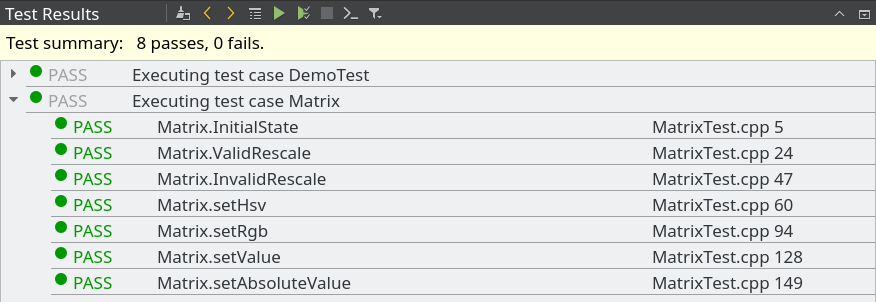
\includegraphics[width=1.0\textwidth]{img/qtcreator_test_results}
	\caption[QtCreator Google Test Results]{Google Test Results in QtCreator}
	\label{fig:qtcreator_test_results}
\end{figure}

\subsection{Qt Test}

While the Google Test Framework is well suitable for general C++ code and has its major advantage in being universal for all platforms and types of code, it has some disadvantages when testing more Qt specific functionalities. With Google Test, much boilerplate code is required to test the Qt Signal\&Slot mechanism for instance.

To overcome these issues we also looked at the Qt Test Framework and evaluated whether it solves them.

\subsubsection{Setup and Test Driver}

Setting up the Qt Testing Framework does not require any additional libraries to be installed (assuming one uses the QtCreator IDE, as we did). However, setting up the test driver requires more code as for the Google driver because the tests can not be found automatically. This is not necessarily a bad thing as it opens up a more flexible test configuration, but may also be more error prone.

The test driver we use for the tests looks like this:

\bigskip
\begin{lstlisting}[title=tests-qt/main.cpp]
#include <QtTest>

#include "MatrixTest.h"
#include "OscNetworkManagerTest.h"
#include "BlockCreationTest.h"

int main(int argc, char** argv) {
	QApplication app(argc, argv);	
	QList<QObject*> testCases;
	testCases << new MatrixTest();
	testCases << new OscNetworkManagerTest();
	testCases << new BlockCreationTest();
	
	int returnValue = 0;
	for (QObject* testCase: testCases) {
		returnValue = returnValue | QTest::qExec(testCase, argc, argv);
	}
	return returnValue;
}
\end{lstlisting}
\bigskip

\subsubsection{Example Test}

Implementing test cases follows the \textit{convention over configuration} approach. For each group of test cases a custom class that inherits from QObject has to be created. To prepare a set of test cases, the method \texttt{initTestCase()} can be declared and is executed automatically by Qt Test before any test case is executed. The method \texttt{cleanupTestCase()} handles the opposite case of cleaning up after the execution of all tests. \texttt{init()} and \texttt{cleanup()} work in the same fashion, but are executed again before each single test case. An example class that declares all these methods can be seen here:

\bigskip
\begin{lstlisting}[title=tests-qt/ClassUnderTest.h]
#pragma once

#include <QtTests>

class ClassUnderTest : public QObject {
	Q_OBJECT
private slots:
	// Will be called before the first test function is executed.
	void initTestCase();
	
	// Will be called after the last test function was executed.
	void cleanupTestCase();
	
	// Will be called before each test function is executed.
	void init();
	
	// Will be called after every test function.
	void cleanup();
}
\end{lstlisting}
\bigskip

Each additional method of the test class which's name starts with 'test' is considered as a test case and is found by Qt with the introspection feature of QObjects.

A very simple test case like in the Google Test example would look like the following:

\begin{lstlisting}[title=tests-qt/Demo.cpp]
void testDemo() {
	QCOMPARE(1+1, 2);
}
\end{lstlisting}

\subsubsection{Differences to Google Test}

\paragraph{Simulating Mouse and Keyboard}

The controllability of GUI tests is much increased by Qt Tests as it offers the functions \texttt{keyClick()} and \texttt{mouseClick()}. They simulate keyboard and mouse events by sending internal Qt events instead of hijacking the input device on operating system level, which means that there are much less side effects when using them. 

Sequences of inputs can be specified and the delay between them adjusted by command line parameters. This makes it quite easy to test custom GUI objects like in our application in an isolated and reproducable way.

\paragraph{Testing Signals and Slots}

To increase the observability, Qt Test provides the class QSignalSpy. It makes it possible to include the amount of signal emission in the expected output of a test and even compare the parameter values of the emitted signals.

In addition, QSignalSpy can start an event loop inside of a test to be able to detect signals that are send between threads using queues or that are emitted with a short delay. The event loop is quited after a specified timeout and the test is considered failed if the expected behavior was not observed in the meantime.

Beside that, it is possible to log all emitted signals with the '-vs' command line parameter, which makes debugging much easier. It also allows to detect unnecessarily repeated signals, which also caused problems in our project before.

\paragraph{Microbenchmarks}

It is possible to include microbenchmarks directly inside the tests. A reasonable number of iterations is detected automatically while running the tests, the type of time measurement can be chosen and the results are reported right after the corresponding test results. Why this is important for GUI application development is further discussed in \vref{performance_regression_tests}.


\subsubsection{IDE Integration}

The Qt Test Framework is integrated in the graphical user interface of Qt Creator, too. As with Google Test, you can start all or only individual tests and see the results aggregated in a summary at the bottom of the window. One of the advantages of Qt Tests can also be seen here: the results of the microbenchmarks, including the number of iterations (see \vref{fig:qtcreator_test_results_qt}).

\begin{figure}[h]
	\centering
	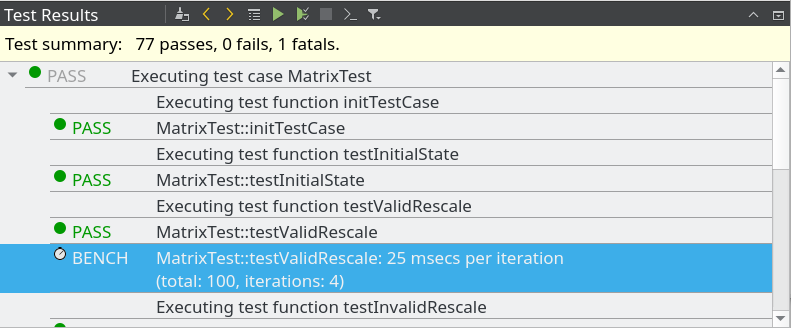
\includegraphics[width=1.0\textwidth]{img/qtcreator_test_results_qt}
	\caption[QtCreator Qt Test Results]{Qt Test Results in QtCreator}
	\label{fig:qtcreator_test_results_qt}
\end{figure}


\subsection{Code Coverage Calculation}

It is not possible to calculate and display the code coverage of tests done with the Google Testing framework or Qt Test within QtCreator.

Fortunately at least the GCC compiler has a compilation option that modifies the program to log the number of times each line of code is executed. The results are stored in separate files next to the executable after the first run of the software and can be analyzed with a tool called \textit{gcov}\footnote{\url{https://gcc.gnu.org/onlinedocs/gcc/Gcov.html}} or visualized as HTML pages with \textit{lcov}\footnote{\url{http://ltp.sourceforge.net/coverage/lcov.php}}. The coverage results for some of the source files in our project can be seen in \vref{fig:test-coverage}.

Even while gcov can only calculate line coverage and not branch coverage or even more complexe coverage criterions, it is already a very useful metric to get insights which parts of the application are tested in an automated way. If the line coverage for some files is under 100\%, for example after a code change, this is a clear indicator that tests are missing.

\begin{figure}[h]
	\centering
	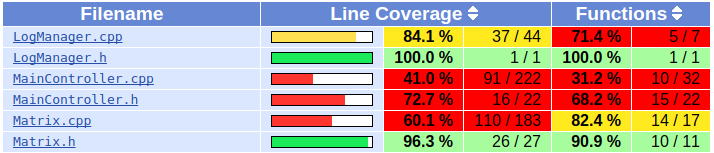
\includegraphics[width=1.0\textwidth]{img/test-coverage}
	\caption[Test Coverage Results]{Test Coverage Results}
	\label{fig:test-coverage}
\end{figure}

% TODO: find out how to calculate (and visualize?) coverage

\subsection{ASA and Testing}

\paragraph{Code Metrics} Metrics generated by ASA like cyclomatic code complexity could indicate error prone code which should be investigated whether exhaustive test cases should be developed.

In our case we used automated static analysis to calculate the cyclomatic complexity for the most crucial parts of the software. However the average complexity was quite low, to be concrete between 3 and 5. High complexity values were mostly a result of switch case statements with many branches and we decided to not design test cases for them.

\paragraph{Test Generation} Another use case of ASA for dynamic testing could be the automated generation of test cases. The only tool we found that claims to do that for C++ code is VectorCAST\footnote{\url{https://www.vectorcast.com/software-testing-products/c-unit-testing}}. It automatically generates test cases by using decision paths, which can be very useful especially for rather large projects as it potentially saves a large amount of time. While it would be interesting to try this for our project, this tool was not available for us.

\section{Evaluation}

\subsection{Bugs Found}
% TODO: mehr beispiele!
Even while writing the first few unit tests, we were able to identify some issues where the code was not behaving as expected.

In the first case an operation was never executed because of a wrong condition in an if-statement (\texttt{rescaleTo()} in Matrix.h).

Furthermore in the same class it was possible to set a variable to a higher or lower value than specified through its setter method. The expected behavior in this case would be that the variable is then limited to its upper or lower bound.

\subsection{Performance Regression Tests}
\label{performance_regression_tests}

The execution time of functions is an especially import aspect in the development of GUI applications. If a function consumes too much CPU time it can not only affect loading times, that can get annoying for the user if they are too long. It can also affect the general perceived responsiveness of the application: the responsiveness is higher if the delays between user interactions and visible changes are kept to a minimum. But in the end on mobile platforms, the most important effect of used CPU time is the battery consumption. When developing an app or in the case of C++ even a part of the operating system, the goal is most of the time to reach the lowest possible power consumption.

A typical way to measure and be able to improve the execution time of single functions are \textit{microbenchmarks}. They measure the used CPU time per function call and summarize the results in a report. The developer can then start identifying performance bottlenecks and fix them.

But in the context of automated testing it would be quite interesting to combine microbenchmarks with tests, especially regression tests.

As most functions in a GUI application have to return in under 20ms for a lag-free user experience, a default timeout of the targeted frame time should be available. Tests that run longer than this duration should be considered failed or at least produce a warning message. The only exception to this are functions that are executed in a dedicated worker thread. It should be possible to mark those functions and disable or increase the timeout for them.

\begin{figure}[h]
	\centering
	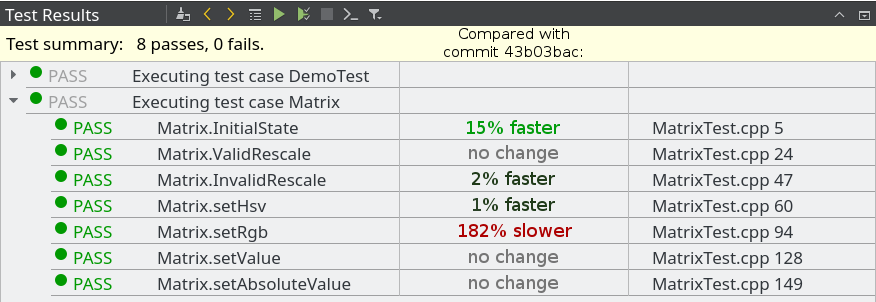
\includegraphics[width=1.0\textwidth]{img/performance_regression_mockup}
	\caption[Mockup: Performance Regression]{\textit{Mockup:} Possible Visualization of Performance Regression Test Results}
	\label{fig:performance_regression_mockup}
\end{figure}

Even better would be the the possibility to run performance regression tests. An overview as proposed in \vref{fig:performance_regression_mockup} could show which of the execution times of tested units increased or decreased after the last change.

This would be very helpful to find regressions in code quality and even misuse of APIs. An example could be that in a bug fix the used sorting algorithm was changed or a linked list was used instead of a vector. A normal unit test would still pass in this case because the output of the function did not change, but only its CPU and memory footprint.

Another example would be the addition of a parameter check to a function as a fix for a failing test. This would seem reasonable to the developer while trying to make all tests pass, but the developer might miss that this function is called million times per second and the parameter checks were removed intentionally because the functions was revealed as a performance bottleneck beforehand. An automated performance regression tests could easily show the effects of the change to the rest of the code and a more speed friendly fix could be found for the failing test.

In reality, an unusually long execution time is often also caused by a large amount of generated debug or warning messages, which is a good indicator for a bug, too.

An overview of aggregated performance changes over many commits and releases could be a good candidate as an indicator for general project health, too. The developers could be motivated to reach a performance improvement in each release by trying to make the report appearing in green, while of course the readability of the code should still have the highest priority in most cases.

Unfortunately we could not find a feature like this in any of the regarded testing frameworks. Qt Test has the ability to include simple benchmarks in the tests but can not compare the results to those of prior commits. Google Test does not even have the ability built in to make benchmarks while testing. While Google offers a separate benchmarking framework for C++ to solve some of the mentioned issues, it is not easily possible to create regressions overviews, either.

To realize performance regression tests, they would need to be executed each time on the same machine and under the same conditions, or the results would need to be normalized in respect to a prior general performance measurement. But in regard of the possible benefits this seems to be a solvable problem.


\chapter{Verification}

Within the next chapter, we will present and discuss different approaches of verifying properties within a given piece of code. The main focus will be directed towards various tools, which support different strategies of verification.

\section{Test Case Generation}

The first of these strategies is to generate test cases automatically. This is especially useful, if exhaustive testing is not an option. Therefore, we rely on methods such as symbolic execution to find crucial edge cases and other important inputs, which might lead to unexpected behavior of our software. If done correctly, the generated test cases can prove some properties of the verified code.

We started searching tools specialized in verifying C++ code. However, we realized that tooling support for C++ is rather rare within the public domain. Additionally, many of the tools we found were outdated and no longer maintained, making it impossible to use them with our modern C++ code. The only tool we were able to use for our C++ code was Polyspace.
In order to find some more tools we could test, we started looking for other supported languages. We found KLEE\footnote{\label{klee_reference}\url{http://klee.github.io/}, accessed 25th January 2018}, a symbolic execution tool for C. Additionally, we tried IntelliTest\footnote{\url{https://docs.microsoft.com/en-us/visualstudio/test/intellitest-manual/introduction}}, another symbolic execution tool for C\#. We had to translate our code to valid C and C\# code when trying these tools, which limited the amount of code we could verify. Therefore, we decided to translate and test our \texttt{HSV} to \texttt{RGB} conversion method.
At this point, we would like to mention that translating code comes with the risk of changing the behavior. Thus, the correctness of the translation must be proven in order to completely verify the given code. However, we verified our code only for the sake of finding and using the above mentioned tools, and therefore, we will not prove that our translation is correct.

\subsection{KLEE}

"\emph{KLEE is a symbolic virtual machine built on top of the LLVM compiler infrastructure [...]}"\footref{klee_reference}


We installed KLEE on a virtual Ubuntu machine, using the pre-build docker image provided in their manual. We had to modify our code translation, telling KLEE which variables should be tested (\texttt{klee\_make\_symbolic}). We ended up with following code:

\begin{lstlisting}[language=C, firstnumber=21]
void hsvToRgb(float h, float s, float v, float* r, float* g, float* b) {(*@\Suppressnumber@*)
	[...](*@\Reactivatenumber{46}@*)
}

void main(int argc, char** argv) {
	float r = 0.f;
	float g = 0.f;
	float b = 0.f;
	
	float h = 0.f;
	float s = 0.f;
	float v = 0.f;
	
	klee_make_symbolic(&h, sizeof(h), "h");
	klee_make_symbolic(&s, sizeof(s), "s");
	klee_make_symbolic(&v, sizeof(v), "v");
	
	hsvToRgb(h, s, v, &r, &g, &b);
}
\end{lstlisting}
\bigskip

We compiled the code, using the included Clang compiler and enabled the \texttt{-emit-llvm} flag, so that KLEE could operate on the result.
Afterwards, we executed KLEE as follows:

\bigskip
\begin{lstlisting}[language=bash, numbers=none, frame=single]
~/verification$ klee Matrix.bc
KLEE: output directory is "/home/klee/verification/klee-out-0"
KLEE: Using STP solver backend
KLEE: WARNING ONCE: silently concretizing (reason: floating point) expression (ReadLSB w32 0 s) to value 0 (/home/klee/verification/Matrix.c:24)

KLEE: done: total instructions = 58
KLEE: done: completed paths = 1
KLEE: done: generated tests = 1
\end{lstlisting}
\bigskip

Unfortunately, KLEE does not support floating point numbers, resulting in just one test case being generated.

\bigskip
\begin{lstlisting}[language=bash, numbers=none, frame=single]
~/verification$ ktest-tool klee-last/test000001.ktest
ktest file : 'klee-last/test000001.ktest'
args       : ['Matrix.bc']
num objects: 3
object    0: name: b'h'
object    0: size: 4
object    0: data: b'\x00\x00\x00\x00'
object    1: name: b's'
object    1: size: 4
object    1: data: b'\x00\x00\x00\x00'
object    2: name: b'v'
object    2: size: 4
object    2: data: b'\x00\x00\x00\x00'
\end{lstlisting}
\bigskip

The test case consists of zeros for all input values, which is not very helpful for verifying properties within our translated code. Thus, we did not further investigate KLEE.

\subsection{Visual Studio Intelli Test}

\begin{itemize}
	\item testing of managed C-Sharp code (.NET framework must be target platform, no x64 support)
	\item translated our \texttt{void hsvToRgb(...)} to C-Sharp and generated test cases
	\item added some assertions and assumptions for better results with Pex
\end{itemize}

\begin{lstlisting}[language=C]
[PexMethod]
public void HsvToRgbTest([PexAssumeUnderTest]Matrix target,
	float h,
	float s,
	float v,
	out float r,
	out float g,
	out float b
)
{
	PexAssume.IsTrue(h >= 0.0f && h <= 1.0f);
	PexAssume.IsTrue(s >= 0.0f && s <= 1.0f);
	PexAssume.IsTrue(v > 0.0f && v <= 1.0f);
	
	target.HsvToRgb(h, s, v, out r, out g, out b);
	
	PexAssert.IsTrue(r >= 0.0f && r <= 1.0f);
	PexAssert.IsTrue(g >= 0.0f && g <= 1.0f);
	PexAssert.IsTrue(b >= 0.0f && b <= 1.0f);
}
\end{lstlisting}

\begin{figure}[h]
	\centering
	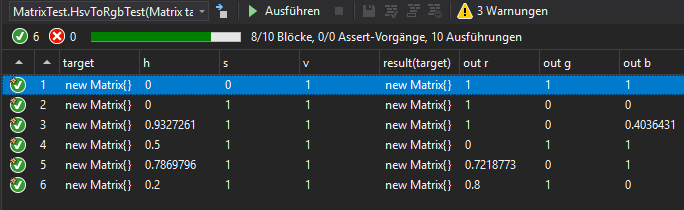
\includegraphics[width=0.75\textwidth]{img/matrix_intelli_test.PNG}
	\caption[Intelli Test Results]{Intelli Test Results}
	\label{fig:matrix_intelli_test}
\end{figure}

\section{ASA without Optimistic Inaccuray}

\begin{itemize}
	\item PolySpace claims not to have optimistic inaccuracy for some kind of faults like nullptr dereferencing, it uses symbolic execution among other techniques
	\item compilers don't have optimistic inaccuracy for some cases (?)
\end{itemize}

\subsection{Polyspace}

Polyspace can analyze code and prove the absence or existence of run time errors by using abstract interpretation.

The detected issues are separated in four categories\footnote{\url{https://www.mathworks.com/products/polyspace-code-prover/features.html}}:
 \begin{itemize}
 	\item \textbf{Green:} proven free of run-time errors
 	\item \textbf{Red:} proven faulty each time the operation is executed
 	\item \textbf{Gray:} proven unreachable (may indicate a functional issue)
 	\item \textbf{Orange:} unproven operation may be faulty under certain conditions
 \end{itemize}

The detected issues for our code example (hsv2rgb) can be seen in \vref{fig:polyspace_categories}.

\begin{figure}[h]
	\centering
	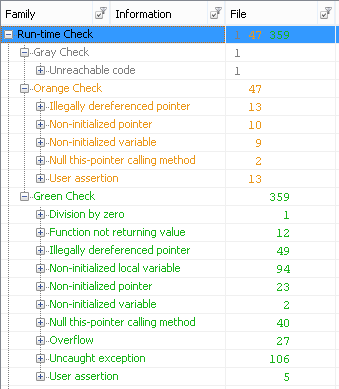
\includegraphics[width=0.5\textwidth]{img/polyspace_categories}
	\caption[Polyspace Code Prover Categories]{Polyspace Code Prover Categories}
	\label{fig:polyspace_categories}
\end{figure}

Furthermore Polyspace can show the possible value range of each variable at every given time as a result of the automatic symbolic execution. These information can also be very useful for debugging, an example can be seen in \vref{fig:polyspace_symbolic_execution}.

\begin{figure}[h]
	\centering
	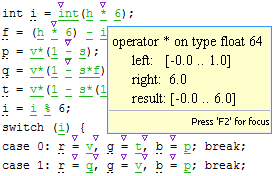
\includegraphics[width=0.5\textwidth]{img/polyspace_symbolic_execution}
	\caption[Symbolic Execution in Polyspace]{Symbolic Execution in Polyspace}
	\label{fig:polyspace_symbolic_execution}
\end{figure}

Polyspace can also display useful information about the state variables in each line of code, for example if it could be null (see \vref{fig:polyspace_variable_information}).

\begin{figure}[h]
	\centering
	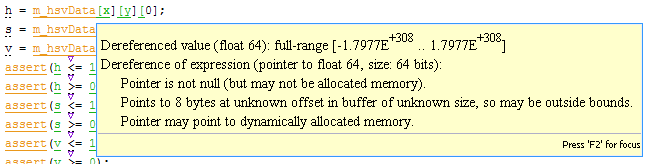
\includegraphics[width=1.0\textwidth]{img/polyspace_variable_information}
	\caption[Polyspace Variable Information]{Polyspace Variable Information}
	\label{fig:polyspace_variable_information}
\end{figure}

Unfortunately it is very hard to compile code with complex dependencies (like Qt) in Polyspace and we had to rewrite the \texttt{hsv2rgb()} function with pure C++ code and STL containers. This may introduce new errors and it may behave differently compared to the Qt container classes.

\section{Theorem Proving}

\begin{itemize}
	\item would be useful for: network protocols (why?), color conversions?
	\item sometimes it is enough to prove a weaker theorem, for color conversions it is often enough that they convert a valid color to another valid color, but not whether it is the correct color
	\item there are no security concerns or sensible data in our application -> demand for verification is rather low
\end{itemize}



\end{document}
